\chapter{Reorganization of brain networks throughout development}

\section{Motivation}

In the previous chapter, we established that reading does not appear to be ``simply'' a change in sensory systems. There are also more global changes in the degree of integration of different RSNs, especially those related to attention and executive control. However, this analysis was conducted in emerging readers: the participants were approximately 10 years old and were at a point in their education where basic skills were in place, but they were still relatively inexperienced readers.
% Age-related differences in structural / functional connectivity \citep{BetzelSporns2015}... 

John Steinbeck stated that, ``Learning to read is probably the most difficult and revolutionary thing that happens to the human brain, and if you don't believe that, watch an illiterate adult try to do it.''


One purported benefit of brain modularity is ``evolvability'': the capacity for a system to easily adapt to environmental circumstances because new modules can be added without drastically altering the other modules \citep{Kashtan2005}. Each one can work in parallel, sharing information when necessary, but without being too dependent on the success or failure of another system. This makes modularity not only efficient but also robust to damage. Cognition, too, has traditionally been considered to a large degree modular, with the pseudo-science of phrenology being the most extreme example, but more recent efforts coming from a deeper understanding of visual and sensory systems \citep{Barrett2006}. However, some higher-order cognitive functions such as working memory, attention and planning have not been localized to a discrete cortical area and are more likely to depend on a global ``workspace'' \citep{Dehaene1998}.

The cognitive processes in reading are also thought of in a modular sense: visual, auditory, semantic and motor processes can each be taught or assessed separately \citep{Cutting2009a}. Phonics instruction spends a great deal of time making individuals better at merging, specifically, the auditory and visual modules. Neuroimaging evidence from the past two decades suggets that this binding process localizes onto the left temporo-parietal junction \citep{}. 

The degree of reorganization is likely to depend on the individual's ability to respond to a given task. Although it is still an area of investigation, one group investigated how modularity changed over the course of learning a novel task. Bassett and colleagues scanned participants at four timepoints while they were learning a new finger-tapping task: before training, early in training, midway through training and at the end of training \citep{Bassett2015}. The authors empirically defined a visual and motor module, and investigated changes to it throughout training. They found two important trends: first, the two modules became increasingly segegated throughout training and practice; and second, the involvement of non-module nodes such as those in subcortical systems was reduced over time. A separate study found that that modules are more likely to re-organize at early stages in the training process \citep{Bassett2010}. Taken together, the findings suggest a model in which the early stages of training require a high degree of cross-module communication, whereas later stages rely on more automated, modular processes (i.e. efficient and segregated processing). 


It could be that the differences between the modalities were due to active support processes that were occuring between executive and attention regions, as the participants performed reading, a relatively novel task. On the one hand, advocates of a ``parallel'' model might assert that additional cognitive processes are used to ``bootstrap'' reading skill at early ages, so that differences between the two systems should decrease with maturity and reading experience as the two systems merge. On the other hand, the ``parasitic'' model of reading would predict that differences would persist, or even become exaggerated, as the two systems become more efficient for their respective tasks. In this chapter, then, we seek to replicate these results in a new cohort of subjects with a different set of passages, and then to investigate the effects of developmental maturity on the reorganizaton of brain networks during reading and listening.

There were two primary motivations in this study:

\begin{itemize}
	\item Which areas ``converge'' and ``diverge'' throughout development?
	\item What shifts in connectivity patterns do we see?
\end{itemize} 

We sought to address four questions:
1. How does modularity (at rest) change over development?
2. Is the modularity / TOWRE correlation consistent in Grades 3 and adolescence?
3. Were there changes in the re-wiring diagram?
4. How does similarity across the many different task states change across age?



To address this, 

\section{Methods}

\subsection{Participants}

To observe changes at multiple points in development, participants in this study were drawn from several study populations and age groups. They fell into three categories: a group of children (ages 8 to 10) were selected from the third wave of the longitudinal study described in Study 1;  a group of adolescents (ages 11 to 14) from a large, cross-sectional study on the cognitive components of reading; and a group of adults (ages 18 to 40), largely from a population of university research assistants and graduate students. In this final group, behavioral data was sparsely collected, so no analyses of reading-related skill are possible. Demographics for these subjects are described in Table \ref{table:ch5-participants}.

\begin{table}[t]
	\renewcommand{\tabcolsep}{0.09cm}
	\centering
	\begin{tabular}{lll}
\toprule
Measure &               Young Group &               Mature Group \\
\midrule
Subjects                        &              38 &              38 \\
Total scan runs                 &             118 &             136 \\
Mean age                        &     9.38 (0.31) &    19.16 (7.99) \\
Sex                             &      18 M, 20 F &      21 M, 17 F \\
Individuals with Testing		& 			  38 &				18	\\
WASI Full-Scale IQ, Vocabulary  &   55.37 (11.95) &    55.89 (7.52) \\
Test of Word Reading Efficiency &  109.95 (15.23) &  101.33 (15.50) \\
\bottomrule
\end{tabular}
	\caption[Participant demographics for Study 4.]{Participant demographics for Study 4. Participants were drawn from three samples: children from the third wave of the longitudinal study described in Studies 1 to 3; adolescents in a cross-sectional study of reading comprehension skill; and adult volunteers. Scan sessions followed the same task design as in Study 3 but stimuli were novel.}
	\label{table:ch5-participants}
\end{table}

\subsection{Functional MRI acquisition and processing}

The task design for this study is described in detail in Chapters 3 and 4. Briefly, subjects were presented up to four separate runs of a language comprehension task. The task included two passage blocks (``Reading'' or ``Listening''), two sensory baseline blocks (``Attention'') and a trailing resting-state block ("Rest"). The four scan runs were crossed on two conditions: the modality of presentation (auditory or visual) and the genre of the passage (narrative or expository). One difference, however, was that the contents of the passages presented to these participants differed from those previously described. While still balanced to a third-grade reading level using Coh-Metrix, the passages were novel. 

Motion is a major confound in age-related connectivity analyses since, on average, children move much more during a given scan session than their older counterparts. To combat this, we applied a stricter motion criteria for inclusion than previously: subjects needed to have no more than 10 percent outlier volumes. A total of 72 unique subjects and 256 scan sessions met this criteria. 

Functional MRI acquisition and preprocessing procedures were equivalent to those described for Studies 2 and 3. See the \textit{Methods} section of Chapter 3 for a detailed description of these processes and their parameters.

\subsection{Activation and network analyses}

Our main questions  was broken into two parts: first, comparing the similarities and differences in network organization for listening and reading, then across all available tasks. 

For the modality comparisons, we used a fixed-effects subject-level model to estimate the shared activation for ``Listening and Reading'' and their differences ``Listening vs. Reading''. We then used FSL's \textit{randomise} utility to estimate the main effects of modality across all subjects in our sample (5000 permutations, threshold-free cluster enhancement, $p < 0.05$).  We also investigated these effects in ``connectome space'' by extracting the values at each of the 264 nodes used for connectivity analysis, then comparing the activity profile of each RSN during reading and listening.

\section{Results}

% Scan inclusion

% Modularity across time and modality age
We first tested the effects of task condition and age on estimates of modularity on the reading comprehension task. We set up a two-way ANOVA with the three groups (young readers, adolescents, adults) as one facto and the three experimental conditions (rest, attention, reading) as the other factor. Figure \ref{fig:ch5-modularity-by-condition-3groups} displays the distribution of these data. 

\begin{figure}[t]
	\centering
	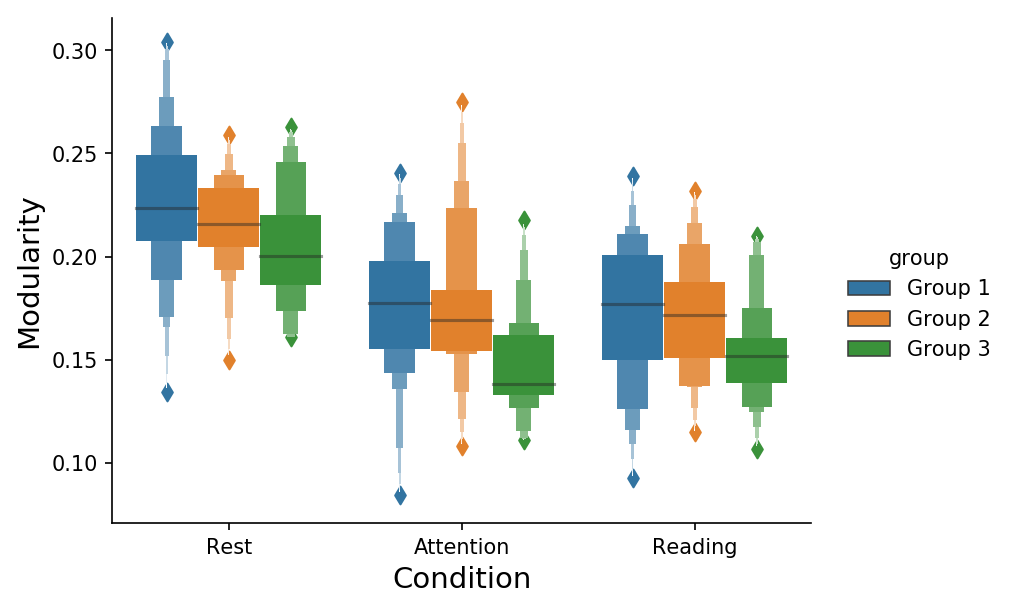
\includegraphics[height=3in]{ch5-modularity-by-condition-3groups}
    \caption[]{}
	\label{fig:ch5-modularity-by-condition-3groups}
\end{figure}

We found significant effects for both group ($F=11.376$, $p < 0.001$ and condition ($F = 60.4$, $p < 0.001$), but not their interaction ($F=0.470$, $p = 0.758$). We then conducted post-hoc $t$-tests on the comparisons within each factor. For group, adults ('Group 3') had a lower modularity than the younger participants, but Groups 1 and 2 were not significant different. For experimental conditions, resting state had a higher modularity than both task conditions, which did not differ significantly. See Table \ref{table:ch5-modularity-age-condition} for specific statistical results.

\begin{table}[t]
	\renewcommand{\tabcolsep}{0.09cm}
	\centering
	\begin{tabular}{lrrrr}
\toprule
Variable &    Sum. of Squares &     Deg. Freedom &          $F$ / $t$ &        $p$-value \\
\midrule
\textsc{Two-Way ANOVA} 	& 	& & & \\
Group                   &  0.023 &    2 &  11.374 &  $< 0.001$ \\
Condition               &  0.126 &    2 &  60.402 &  $< 0.001$ \\
Group:Conditions 		&  0.001 &    4 &   0.469 &  $0.758$ \\
Residual                &  0.229 &  219 &        --- &           --- \\
& & & & \\
\textsc{Post-Hoc $t$-tests} & & & & \\
\textit{Conditions} & & & & \\
Rest > Attention  	&  ---  &    ---- &  13.341 &  $< 0.001$ \\
Rest > Reading  	&  ---  &    ---- &  14.279 &  $< 0.001$ \\
Attention > Reading &  ---  &    ---- &  0.437 &  $0.663$ \\
\textit{Groups} & & & & \\
Group 1 > Group 2  &  ---  &    ---- &  0.604 &  $0.546$ \\
Group 1 > Group 3  &  ---  &    ---- &  3.733 &  $< 0.001$ \\
Group 2 > Group 3  &  ---  &    ---- &  2.869 &  $0.005$ \\
\bottomrule
\end{tabular}
	\caption[Statistical results for the effects of condition and group on modularity.]{Two-way ANOVA table for the main effects of condition and group on modularity. Below are results for post-hoc $t$-tests conducted within each factor.}
	\label{table:ch5-modularity-age-condition}
\end{table}

% Modularity to reading
Next, we attempted to replicate our findings that higher modularity at rest was associated with higher reading skill. We were unable to test the comparison in the oldest readers (ages 15 and older), but we did have TOWRE scores from an older sample of children and the adolescents in Group 2. When all subjects were included in the analysis (n = 56), there was a positive correlation that trended toward significance but did not reach it ($r = 0.256$, $p = 0.057$). When analyzed separately, the correlation was higher in younger readers ($r=0.280$, $p=0.089$) than older readers ($r=0.198$, $p=0.432$). 

\begin{figure}[t]
	\centering
	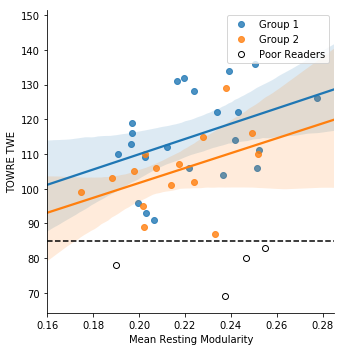
\includegraphics[height=3in]{ch5-modularity-reading-corr-2groups}
    \caption[]{}
	\label{fig:ch5-modularity-reading-corr-2groups}
\end{figure}

% Excluding the lowest subjects
We noticed that some of the poorest readers had more variability in their modularity values. We re-ran the correlations excluding the readers with standard scores of 85 or less (one standard deviation below average, or the bottom 16 percent). This significantly improved the correlation across the entire group ($r = 0.404$, $p = 0.003$) and the younger group ($r = 0.459$, $p = 0.006$). Although the correlation increased for the older group, it did not reach significance either ($r = 0.292$, $p = 0.273$).

% Similarity betwen listening and reading over time
Finally, we investigated how subject ``flexibility'' changed over time. We first compared the degree of subject similarity between ``developing readers'' (Group 1) and ``mature readers'' (Groups 2 and 3) during reading and rest. Consistent with our findings of decreased modularity, we found that older readers had, on average, lower similarity to their peers than children did ($t=...$). 

Within each individual subject, however, there was no change in the degree of ``flexibility'' -- the amount of variance seen between different conditions ($t = ...$... ). This suggests that   Despite the findings of decreased modularity, we found that no evidence that the mean IOU across all conditions was actually no different across any of the groups.
This pattern of results suggests that, as you grow, you develop a more unique pattern

% Similarity across all conditions over time
To investigate whether this could be explained in terms of mean trends, we ...


\begin{figure}[t]
	\centering
	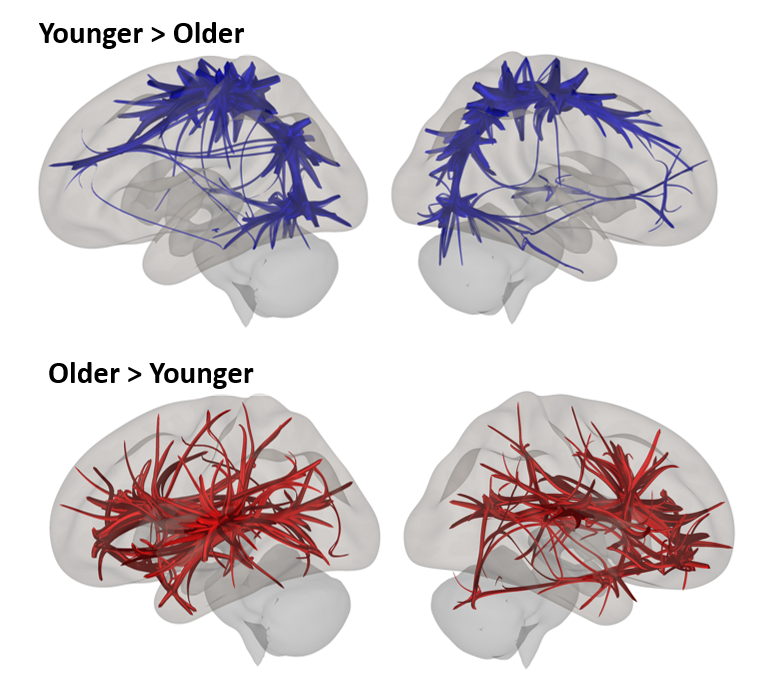
\includegraphics[height=3in]{ch5-group-difference-connections}
    \caption[]{}
	\label{fig:ch5-group-difference-connections}
\end{figure}


\begin{figure}[t]
	\centering
	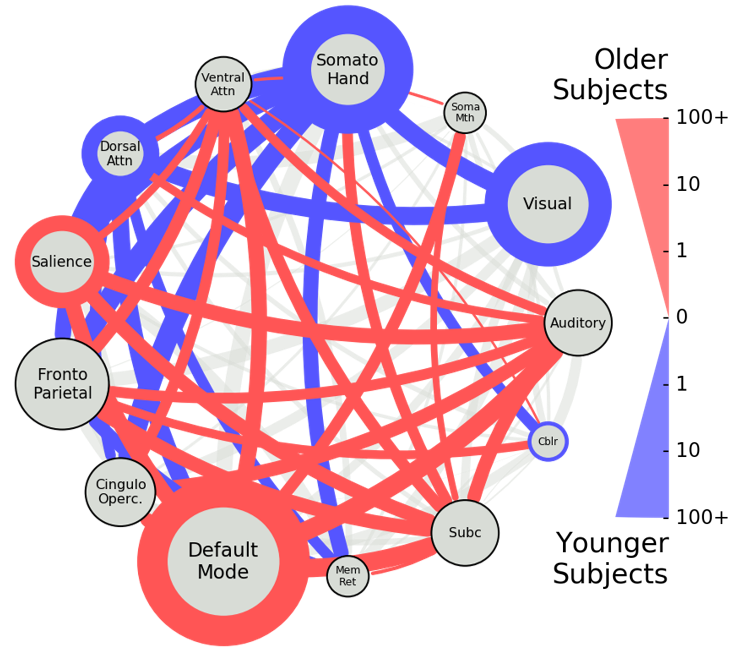
\includegraphics[height=3in]{ch5-group-difference-rsn-connectivity}
    \caption[]{}
	\label{fig:ch5-group-difference-rsn-connectivity}
\end{figure}

\section{Discussion}



% \begin{figure}[t]
% 	\centering
%     \caption[Relationship between activation in visual word form area and age.]{}
% \end{figure}

% \begin{figure}[t]
% 	\centering
%     \caption[Global participation coefficient as a function of age.]{}
% \end{figure}